\chapter{Particionamento}



\section{Visão Geral Sobre o Problema de Particionamento}

A decomposição de um design de referencial de \textit{\textit{software}} pode gerar dois componentes: uma porção a ser realizada em \textit{hardware} e outra executada em \textit{software}, num processador e isso é chamado de problema de particionamento. Para sistemas baseados em Plataformas FPGA, particionamento é um subproblema de um problema mais geral localizado no codesign de \textit{hardware} e \textit{software}. 

Para início, será considerado uma aplicação como um conjunto de instruções organizadas como uma coleção de grafos de fluxo de controle especificando a ordem de execução. Sendo assim, a ideia do particionamento é o grupo de específicos conjuntos de instruções em uma aplicação e então mapear esses grupos tanto em \textit{hardware} e \textit{software}. Os grupos designados ao \textit{software} são executados sequencialmente enquanto os mapeados em \textit{hardware} são implementados por uma combinação customizada ou por circuitos sequenciais. Se uma aplicação é totalmente funcional em design referencial de \textit{software}, o resultado do particionamento é conhecido como decomposição. Alguns fatores podem ajudar nas decisões de particionamento tal como expectativa de ganho de performance, os recursos utilizados em \textit{hardware}, como são usados e talvez o mais importante quanto de sobrecarga de comunicação a decomposição impõe ou dificuldade de implementar um conjunto específico em \textit{hardware}.

Recurso por definição são instruções de um \textit{cluster} conectado de aplicações de design referencial de \textit{software} adequado para uma implementação de \textit{hardware}. Adequado será utilizado para definir `o projetista do sistema antecipa que uma implementação de \textit{hardware} se mostrará vantajosa’. Para obter uma boa partição, geralmente tem que examinar grupos que podem ser maiores ou menores que sub-rotinas definidas pelo programador. Recurso pode variar de um pequeno conjunto de instruções para um \textit{kernel} de loops aninhados até um modulo de \textit{software} completo consistente de múltiplas sub-rotinas. Como o tamanho dos recursos afetam na performance, a decisão de implementação em \textit{hardware} depende da sua melhoria no sistema por inteiro e os recursos utilizados relativos a outros recursos candidatos. Se determinado a ser valido a pena, então os recursos de implementação em \textit{hardware} aumentam a arquitetura de \textit{hardware}. 

\textit{Profile}, também conhecido como recorte, é uma técnica para coletar informações em tempo de execução de uma aplicação. O \textit{software} referencial é executado com uma entrada representativa e o tempo gasto em várias partes da aplicação é mensurado. Um exemplo é exibido na Figura \ref{fig:f4-1} onde exibe a codificação de uma imagem.

\begin{figure}[h] \centering
	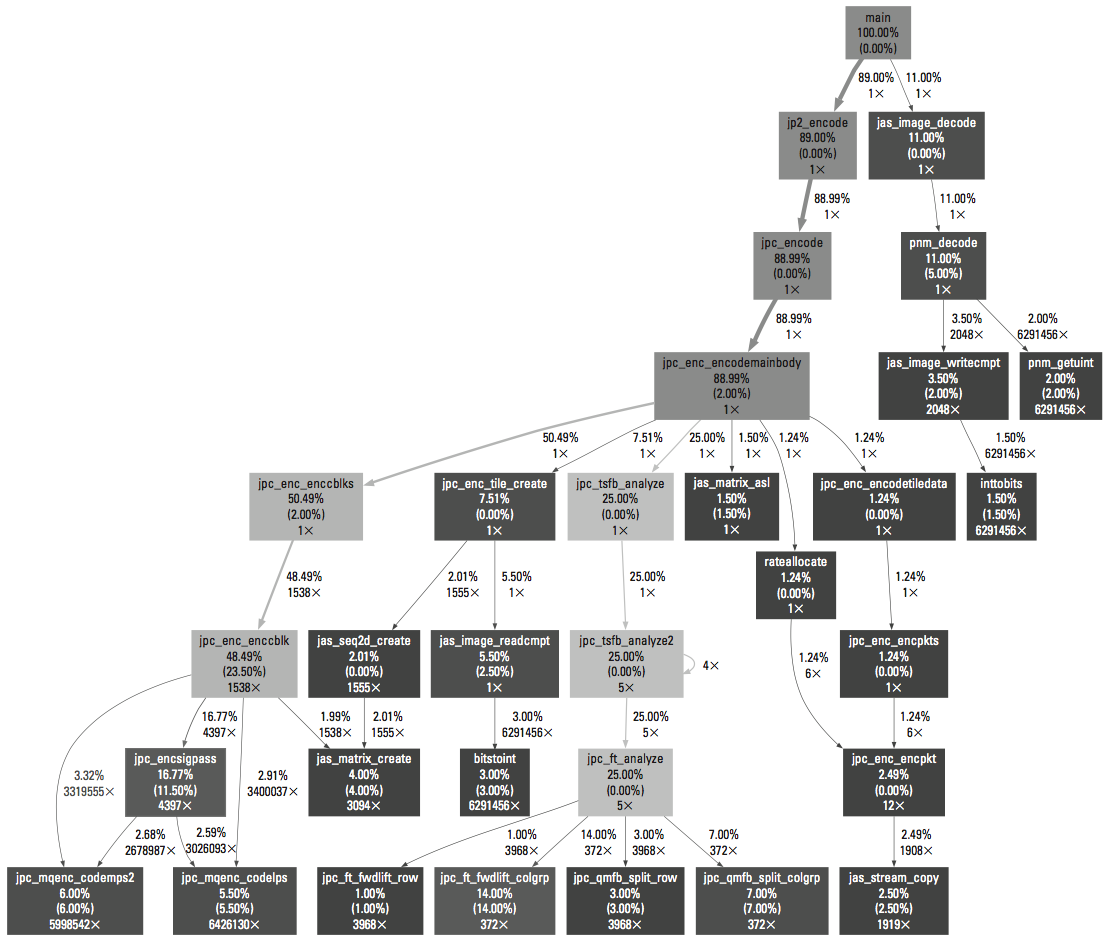
\includegraphics[width=0.9\textwidth]{img/f4-1.png}
	\caption{}
	\label{fig:f4-1}
\end{figure}

Aqui será assumido a técnica simplista que recortará uma aplicação por interrupção periódica e amostrar o \textit{program counter}. Um histograma pode ser utilizado para contar quando um programa é interrompido em um endereço particular e a partir desse, uma fração aproximada do tempo total de execução gasto em várias partes da aplicação pode ser computado.

A análise de performance é definida pela Lei de Amdahl que aplica a lei de retornos decrescentes à utilidade de uma única arquitetura, ou seja, 



$$ \text{Speed up}_{overall} = \frac{1}{(1 - \text{Fraction}_{enhanced}) + \frac{\text{Fraction}_{enhanced}}{\text{Speed up}_{enhanced}}} $$



articulando os limites de um melhoramento geral para uma aplicação que um simples realce pode fazer em tempo de execução. Generalizando para incluir todos os potenciais realces e métricas de performance arbitrária, pode-se caracterizar os limites como coleções de realce. Se forem em recursos de \textit{hardware} e pode-se antecipar que requer ganho potencial de recursos para cara tal, então pode-se desenvolver um modelo que irá orientar ao processo de particionamento. Tal lei não é adequada pois:
\begin{itemize}
\item Visa um simples realce e não nos auxilia a selecionar um subconjunto de uma coleção de recursos potenciais;
\item Foca somente no tempo de execução;
\item Não visa recursos requeridos;
\item Não visa custo de comunicações.
\end{itemize}

Perfis baseados em exemplos requerem representações de entrada e é uma aproximação de tempo gasto. Sem implementar todo o potencial de recursos em \textit{hardware}, pode ser difícil antecipar os recursos requeridos. Pode-se com determinação analítica calcular quantos ciclos de \textit{clock} um recurso de \textit{hardware} irá tomar, podendo assim calcular métricas como \textit{speed up}. Entretanto, é impossível saber quando um processo arbitrário será completado. Ao invés de prover uma solução automatizada, a solução analítica simplesmente provê um \textit{framework} para guiar um designer de sistema a criar uma solução criativa.



\section{Solução analítica para particionamento}

Para definir o problema, será descrito fórmulas matemáticas do problema de agrupamento de instruções em recursos e então os seus mapeamentos em \textit{hardware} ou \textit{software} e ao final, converter os recursos em implementações em FPGA. Atualmente, a forma mais comum de transcrever é descrever manualmente o core com um HDL utilizando design referencial de \textit{software} como especificação.

Muitos problemas práticos impactam na performance atual do sistema. Nem todos os problemas podem ser incorporados a um modelo analítico e por isso podemos caminhar no sentido de soluções matemáticas que irão produzir uma resposta aproximada ao problema de particionamento. Muitas das entradas do nosso modelo são estimadas ou aproximações no qual futuramente degrada a fidelidade de resultados. Deve-se importar com isso pois resolvendo o problema de particionamento `no papel’, tem-se um particionamento que é próximo ao ótimo. Daqui, cabe ao designer ser habilidoso em usar os guias e projetar uma solução mais refinada. Ao final, é mais eficiente usar uma combinação de técnicas \textit{ad hoc} e matemáticas para encontrar uma solução ótima do que simplesmente confiar numa intuição de engenheiro.

Para continuar, deve-se definir alguns conceitos básicos. Sabe-se já de antemão o modelamento de uma sub-rotina de um design referencial de \textit{software} utilizando o grafo de controle de fluxo (CFG) e além desse, será descrito uma nova notação para incluir o grafo de chamada (CG), no qual consiste num conjunto de CFGs, um por sub-rotinas 

$$ \mathcal{C} = {C_0, C_1, \dots C_{n-1}} $$ 

onde $ C_i = (B_i, F_i) $ é o CFG de uma sub-rotina $ i $. Sendo assim, a CG da aplicação é escrita por 

$$ \mathcal{A} \subseteq (\mathcal{C}, \mathcal{L}) $$ 

onde $ \mathcal{L} \in \mathcal{C} \times \mathcal{C} $. Duas sub-rotinas são relacionadas $ (C_i, C_j) pertence \mathcal{L} $ se podem ser determinadas no tempo de compilação que a sub-rotina $ i $ tem potencial de invocar a sub-rotina $ j $.

É assumido que os blocos básicos de cada sub-rotina são disjuntos, ou seja, cada bloco básico em uma aplicação pertence a exatamente um CFG. Além do mais, é assumido que um nó raiz para o CG é implícito, ou seja, uma sub-rotina é designada a iniciar a execução. Nem todos os executáveis podem ser expressados nesse modelo. O manuseio de sinais e interrupções não são representadas e assim, não é possível determinar todos vértices, $ F_i $ em uma dada sub-rotina $ C_i $ de um CFG antes da execução. Finalmente, o paradigma de orientação à objeto depende do tempo de execução para conectar os métodos virtuais invocados. Por design, esse paradigma nos previne de saber todos os vértices antes da execução. Para agora, será considerado que o modelo é suficiente para ser expressado em design referencial de \textit{software}. 

Um equívoco comum é que uma definição formal de particionamento só aplica a separação de aplicação componentes de \textit{hardware} e \textit{software}. Além do mais, para fazer o problema mais tratável é comum agrupar operandos de primeiro recurso, ou seja, uma partição com um grande número de subconjuntos, e então mapeia esses recursos em ambos \textit{hardware} e \textit{software}. Assumindo que esses recursos são razoavelmente bem \textit{clustered}, então a decomposição de uma aplicação em componentes de \textit{hardware} e \textit{software} pode ser dirigido por comparações de ganho de performance de um recurso contra outro.

Primeiramente, definiremos uma partição formalmente. Uma partição $ \mathcal{S} = {S_0, S_1, \dots}$ de um conjunto universal $ U $ é um conjunto de subconjuntos de $ U $ sendo que 

$$ \bigcup_{S \in \mathcal{S}} S = U $$

$$ \forall S, S' \in \mathcal{S} | \mathcal{S} \cap \mathcal{S}' = \emptyset $$

e

$$ \forall S \in \mathcal{S} \cdot S \neq  \emptyset $$

A equação 4.1 diz que cada elemento de $ U $ é um membro de pelo menos um subconjunto $ S \in \mathcal{S} $. A equação 4.2 e 4.3 diz que os subconjuntos $ S \in \mathcal{S} $ são emparelhados disjuntos e não vazio. Em outras palavras, cada elemento do nosso universo $ U $ termina exatamente em um dos subconjuntos de $ \mathcal{S} $ e nenhum dos subconjuntos são vazios. Por exemplo, considere as vogais da língua inglesa onde $ U = {a, e, i, o, u, y} $. Uma partição $ \mathcal{X}_a $ de $ U $ é

$$ \mathcal{X}_a = {{a, e, i, o, u}, {y}} $$

e outro exemplo é 

$$ \mathcal{X}_b = {{a}, {e}, {i}, {o}, {u}, {y}} $$

A Figura \ref{fig:f4-2} ilustra o $ \mathcal{X}_a $ graficamente.

\begin{figure}[h] \centering
	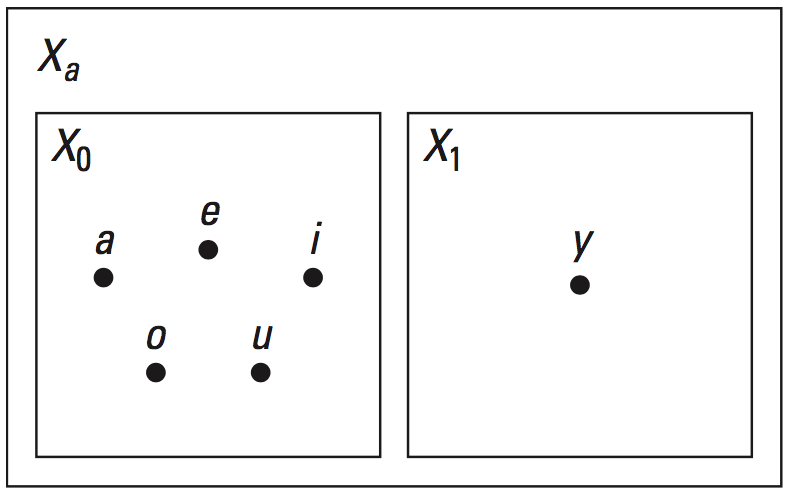
\includegraphics[width=0.5\textwidth]{img/f4-2.png}
	\caption{}
	\label{fig:f4-2}
\end{figure}

Pode-se também aplicar em uma aplicação $ \mathcal{A} $. Se assumirmos que nosso universo é o conjunto de todos os blocos básicos de cada sub-rotina, 

$$ U = \cup_{C \in \mathcal{C}} V(C) $$

então U é as partições de sub-rotinas e chamaremos de partição natural de aplicação onde

$$
\mathcal{S}  = \left \{  
\underbrace{\left \{ b_0, b_1, \dots, b_i \right \}}_{\text{sub-rotine }C_0},
\underbrace{\left \{ b_i, b_{i+1}, \dots, \right \}}_{\text{sub-rotine }C_1},\dots
\underbrace{\left \{ b_j, b_{j+1}, \dots, \right \}}_{\text{sub-rotine }C_{n-1}}
\right \}
$$

Nossa tarefa será reorganizar a partição de blocos básicos e então mapear cada subconjunto de ambos os \textit{hardwares} e \textit{software}. Dessa forma, estamos livres para criar e remover subconjuntos não vazios, e mover blocos básicos ao redor até termos uma nova partição e assim termos um novo resultado $ \mathcal{A}’ = (\mathcal{C}’, \mathcal{L}’) $, inferido a partir da reorganização da partição $ \mathcal{X}’ $. O segundo passo é mapear cada subconjunto de $ \mathcal{X} $ para ambos \textit{hardware} e \textit{software} como é exibido abaixo

$$ 
\mathcal{X}'   = \left \{  
\underbrace{\left \{ b_j, b_{j+1}, \dots, \right \}\left \{ b_k, b_{k+1}, \dots, \right \}\dots}_{\text{software}}
\underbrace{\left \{ b_0, b_1, \dots, b_i \right \} \left \{ b_i, b_{i+1}, \dots, \right \}\dots}_{\text{hardware}}
\right \}
$$



\subsection{Ganho de performance esperado}

Para explicar como performance pode ser utilizado para guiar o particionamento, será utilizado uma métrica simples chamada taxa de execução. É parcialmente motivada pelo fato de que o ganho de performance é relativamente fácil de ser mensurado e por causa de que de todas as métricas comumente utilizadas, \textit{speed up} é frequentemente a mais importante. Diferente do mundo \textit{software} onde tense análise de ordem de complexidade, \textit{hardware} não possui um guia geral para comparação. Ganho de performance para aplicações pode residir em uma acumulação de pequenos ganhos que deveria ser perdido numa aplicação direta na teoria de complexidade. 

Sendo assim, será usado a informação de \textit{profiling} para coletar o tempo total de execução bem com uma fração do tempo gasto em casa sub-rotina. O produto é a aproximação entre o tempo necessário para executar uma porção de aplicação em \textit{software} e usar isso como o tempo que se espera que tomará em futuras execuções. Será utilizado $ s(i) $ para representar o tempo de execução esperado para uma invocação de uma sub-rotina $ i $, ou seja, bloco básico. É uma aproximação para um número de razões, não é o mínimo que depende dos conjuntos de dados de entrada para muitas aplicações. Mesmo assim, existe também exemplos de erros que podem impactar a performance.

Seguindo, precisa-se aproximar o tempo que é uma implementação equivalente em \textit{hardware} que iria tomar. No caso dos blocos básicos, isso é frequentemente mais preciso. Sem fluxo de controle, não presente em blocos básicos, uma ferramenta de síntese pode dar bastante aproximação de acurácia de propagação de tempo. Ou se o recurso é pipelined, o número de estágios é mais precisamente conhecido. Se o recurso inclui fluxo de controle, mas não contém nenhum loop, o caminho mais longo pode ser usado como uma estimativa conservativa. Recursos com um número de variáveis de iterações através de um loop apresentam o maior obstáculo para encontrar um tempo de \textit{hardware} aproximado. Nesse caso, implementação e \textit{profiling} com recurso em \textit{hardware} pode ser a única solução. Independente, assumimos que uma aproximação apropriada $ h(i) $ para o existente tempo de execução em \textit{hardware}.

Finalmente, a interface entre \textit{software} e \textit{hardware} requer tempo e este custo precisa ser contabilizado também. Pode-se aproximar este custo pela aproximação do montante total do estado que necessita ser transferido ou o custo de configuração e latência. Em ambos os caso, são representados por $ m(i) $ para recursos $ i \in \mathcal{H} $.

Taxa de execução é a velocidade na qual um sistema computacional completa uma aplicação, e em um sistema de plataforma FPGA olhamos para o \textit{hardware} para melhorar sua taxa de execução. Esse ganho, no qual comparado com uma solução \textit{hardware} e \textit{software} contra uma solução puramente \textit{software}, é tipicamente mensurada como \textit{speed up}. Utilizamos $ \mathcal{Y} $ para sua representação e isso nos permitira comprar recursos diferentes contra outros para determinar melhores particionamentos. Dessa forma, qualquer subconjunto de blocos básicos que não produzem um ganho de performance, podem ser excluídos geralmente de consideração. Em outras palavras, somente subconjuntos de blocos básicos para qual $ \mathcal{Y} > 1.0 $ são considerados recursos candidatos.

Em geral, não mensuramos taxa de execução, mas ao invés disso, o tempo de execução, que no caso é inverso. Então quando considerando se um conjunto particular de blocos básicos deveriam ser mapeados ao \textit{hardware} ou \textit{software}, estamos interessados em seu ganho em \textit{speed up} ou 

$$ \mathcal{Y} = \frac{\text{hardware speed}}{\text{software speed}} = \frac{\frac{1}{\text{hardware time}}}{\frac{1}{\text{software time}}} = \frac{\text{software time}}{\text{hardware time}} $$

Mais especificamente, estamos interessados no ganho de performance individual de cada recurso e assim, definindo $ \mathcal{Y}(i), i \in \mathcal{C} $

$$ \mathcal{Y}(i) = \frac{s(i)}{h(i) + m(i) } $$

onde $ h(i) $ e $ s(i) $ são o tempo de execução de uma implementação de um recurso $ i $ em \textit{hardware} e \textit{software}. A função $ m(i) $ é o tempo que se leva para sincronização, estado preso, ou seja, o tempo que leva para guiar um dado entre o processador e o item reconfigurável.

Assumindo por um momento que usaremos esse recurso separado em nosso design, deve-se questionar sobre o quão rápido é a aplicação. Isso é dependente em ambos o ganho de performance do recurso e o qual frequentemente é utilizado no design referencial de \textit{software}. Pode-se ter uma fração do tempo gerado em um recurso particular $ f(i) $ a partir de informações de \textit{profile}. Então, o \textit{speed up} da aplicação no geral será

$$ \Gamma = \left [ (1 - f(i)) + \frac{f(i)}{\mathcal{Y}(i)} \right ]^{-1}  $$

A inversão representa que estamos movendo entre tempo de execução e taxa de execução para manter o sentido de ganho de performance.

A partir dessa equação, podemos observar que aumentando a velocidade do \textit{hardware} de um único recurso tem-se menos e menos impacto na performance da aplicação a medida que sua frequência decresce. Para aumentar a performance sistêmica de uma aplicação no geral, também queremos olhar sobre uma outra dimensão: aumentando o sistema com múltiplos recursos que aumentará a performance de componentes individualmente assim como aumentando a fração agregada de tempo gasto em \textit{hardware}. Reconhecendo isso, queremos computar o \textit{speed up} de múltiplos recursos em \textit{hardware}, ou seja, quer-se avalizar o ganho sistêmico de um conjunto de recursos $ \mathbb{D} $ onde cada membro do conjunto contribui à performance do sistema baseado na fração do tempo gasto em cada característica. Para estimar a performance desta partição, podemos adicionar recursos e rearranjar os termos para ter um ganho de performance esperado no geral

$$ \Gamma (\mathbb{D} = \left [ 1 + \sum _{i \in \mathbb{D}} (\frac{f(i)}{\mathcal{Y}(i)} – f(i)) \right ]^{-1} $$



\subsection{Considerações de Recursos}

Seguindo a equação exibida, se tentaria adicionar recursos na abordagem $\sum_i f_i$. Em outras palavras, seria implementar tudo em \textit{hardware} para maximizar a performance, ignorando todos os custos de desenvolvimento e recursos limitados. Num FPGA, há um número finito de recursos disponíveis para implementação de circuitos em \textit{hardware}. Tais recursos são limitados e a maioria das aplicações realísticas irão exceder esse limite disponível. Um meio de aproximação de recursos é contar o número de células lógicas requeridas para cada recurso. Um chip que terá um valor escalar $ r_{FPGA} $ que representa o total de números de células lógicas disponíveis. Então $ r(i) $ pode ser usado para representar a quantidade de células lógicas requeridas por cada recurso $ i $. Uma simples relação 

$$ \sum_{i \in \mathbb{D}} r(i) < r_{FPGA} $$

restringe quão largo $ \mathbb{D} $ pode crescer.

Sabendo que dispositivos modernos são heterogêneos, uma típica plataforma FPGA tem múltiplos tipos de recursos além de células lógicas como memória, blocos DSP, etc. Sendo assim, um vetor seria uma melhor representação

$$ 
\vec{r}_{FPGA} =
\begin{pmatrix}
r_0\\ 
r_1\\ 
\dots \\
r_{n-1}
\end{pmatrix}
$$

Também promovemos a função de requerimentos de recursos para um vetor onde $ \vec{r}(i) $ representa o recurso requerido pelo recurso $ i $. Assim, a nova equação de restrição de recurso é similar 

$$ \sum_{i \in \mathbb{D}} \vec{r}(i) < \vec{r}_{FPGA} $$

onde $ \mathbb{D} $ é o conjunto de recurso incluídos no design.

Infelizmente, esse modelo não toma conta o fato de que alguns recursos alocados podem interferir em outros além de que a estimativa de performance é frequentemente baseada na suposição que recursos são próximos um do outro e recursos de rotas não são parte integral do modelo.



\subsection{Abordagem Analítica}

Já descrito as ferramentas matemáticas necessárias para descrever o problema fundamental do particionamento, pode-se então, primeiramente descrever formalmente o problema em termos de variáveis e descrever um algoritmo para encontrar uma solução aproximada.



\subsubsection{Declaração do problema}

A ideia básica é encontrar um particionamento para todos os blocos básicos de uma aplicação e então separá-los em \textit{hardware} e \textit{software}. Formalmente, procura-se por uma partição $ \mathcal{P} $ de todos os blocos básicos $ U $ de uma aplicação

$$ U = \cup_{C \in \mathcal{C}} V(C) $$

Um subconjunto, $ \mathbb{C} \subseteq U $ onde $ C $ é um vértice de um grafo $ A = (C, L) $ de um design referencial de \textit{software}, é chamado conjunto de candidatos e contem todos os recursos arquiteturais potenciais, ou seja, o subconjunto de $ U $ que é esperado para melhorar a performance do sistema se implementado em um \textit{hardware} reconfigurável. Devido ao limite de recursos, deve-se refinar para o subconjunto $ \mathbb{D} \subseteq \mathbb{C} $ que maximiza nosso métrica de performance

$$ \Gamma ( \mathbb{D}) \text{é maximizado, e } \\ 
\sum_{i \in \mathbb{d}} \vec{r}(i) < \vec{r}_{FPGA}
$$

Algoritcamente, uma abordagem desse problema seria encontrar todas as partições de $ U $, sintetizando e \textit{profiling} cada partição, e então, quantitativamente avalizar cada $ \Gamma $, mas uma aplicação simples que utilizaria cerca de 10 mil blocos básicos, seria mais que $ 10^7 $, significando que o número de partições seria aproximadamente $ 2^{10^{7}} $ e por isso será discutido métodos heurísticos para tal.



\subsubsection{Heurística}

O problema de particionamento é essencialmente uma questão indireta de manipulação de parâmetros $ f(i) $ e $ \gamma(i) $ pelo rearranjo do particionamento $ \mathcal{X} $. Então seleciona-se os elementos de $ X $ que satisfaz as restrições de recurso e maximiza a performance do sistema $ \Gamma $. A heurística pode ser aplicada informalmente para iniciar a partição natural por design referencial de \textit{software}, ou seja, utiliza-se as sub-rotinas de uma aplicação original. Utilizando a ferramenta de \textit{profiling} é listado as sub-rotinas em ordem decrescente em tempo e verificado as que possuem maior valor $ f $. O valor de $ \gamma $ será estimado pela performance esperada a partir da implementação em \textit{hardware} e ao final, tem-se um ganho estimado do sistema para cada sub-rotina.



Em seguida, quer-se manipular iterativamente a partição $ \mathcal{X} = \{ X_0, X_1, ...\} $ criando um novo subconjunto de blocos básicos por meio de operações de casamento e movimentações de blocos. A ideia é procurar mudanças que podem aumentar a fração $ f $ ou o valor de $ \gamma $.



\subsubsection{Fração do Tempo de Execução}

Uma forma de aumentar fração de tempo gasto em uma sub-rotina é tornando maior seu recurso. Isso pode ser alcançado procurando por relações no grafo de chamadas ou, após a manipulação, procurando por relacionamentos no grafo de fluxo de controle que conecta subconjuntos. Por exemplo, supondo que uma aplicação gaste $ 0.5 \% $ do seu tempo, $ f(i) = 0.005 $ numa sub-rotina A e $ 0.025\% $ em uma sub-rotina B e C. A fração de tempo gasto em A pode ser duplicado pelo casamento de A, B e C, entretanto, isso possui seu preço. Geralmente, aumenta-se o número de recursos utilizados e também pode aumentar no tamanho do subconjunto do sistema, decrescendo sua performance.



\subsubsection{Ganho de Performance}

Para aumentar o ganho de recurso $ \gamma (i) $ necessita-se verificar o grafo de fluxo de controle do recurso e avaliar se uma mudança o tornará mais sequencial ou paralelo. Frequentemente, algoritmos que são inerentemente sequenciais possuem melhor performance em processador por este não ter a sobrecarga de configurações de transistores e de possuírem melhor gerenciamento de energia nessas circunstâncias. Simplesmente adicionar blocos básicos pode criar um efeito indesejável de aumentar o comportamento sequencial, reduzindo o $ \gamma $ e criando um recurso menor, pode aumentar seu ganho. Assim, tendo uma sub-rotina $ X $ e quebrando-a em duas sob-rotinas $ X – X' $ e $ X' $, onde a sub-rotina $ X – X' $ invoca $ X' $, então se $ X' $ pode ser melhorado em nível de \textit{hardware} deixando a parte sequencial em $ X – X' $ então $ \gamma $ de $ X' $ será maior e necessitará de mais recursos. Assim, supondo uma sub-rotina tome $ 93\% $ de tempo e provê ganho de $ \gamma = 2 $ então a aplicação terá performance de $ \Gamma = 1.869 $. Entretanto, se uma parte da sub-rotina pode ser extraída aumentando o paralelismo, então é possível que a performance possa chegar a um valor de $ 10 $, $ \gamma = 20 $ enquanto o tempo decresce para $ 83\% $. Esse particionamento gera um \textit{\textit{speed up}} de $ \Gamma = 4.739 $.


Com isso é importante notar que qualquer mudança no subconjunto pode afetar a performance para melhor ou pior. Em geral, heurísticas trabalham examinando os grafos da aplicação e então fazendo mudanças incrementais ao subconjunto de uma partição. Tais mudanças são guiadas pela tentativa de aumentar o tempo gasto em uma sub-rotina não aumentando dramaticamente seus recursos ou decrescendo sua performance; e tentando aumentar a performance sem reduzir o tempo gasto em uma sub-rotina.



\section{Comunicação}

Ao realizar o particionamento, deve-se criar uma comunicação entre os componentes e com isso deve-se discutir o número de questões relacionadas ao estado de comunicação sobre os limites do particionamento e o mecanismo para controle de transferência entre ambos os níveis. Um exemplo disso é uma sub-rotina que realiza a correção de erro bit a bit. É esperado que, como existem operações em bits, a sub-rotina possua melhor desempenho ao ser implementada em \textit{hardware}, tornando-a uma candidata. Inicialmente é posta como uma candidata pois os recursos possuem números limitados e talvez ela não faça parte da decomposição mais benéfica. Uma vez implementada em \textit{hardware}, deve-se realizar a interação entre o recurso e o processador. Sabendo que existem abundância em interfaces padronizadas, em FPGA é possível utilizar uma interface pré-definida ou criar uma nova para cada recurso e essa questão é crucial pois a comunicação também define a performance do sistema.



Adicionar um recurso requer que o processador e o recurso mantenham constante visão dos dados da aplicação. O interfaceamento é o que permite o recurso e o processador comunicar mudanças de estado e é necessário para continuar um dado de aplicação consistente. No desenvolvimento de design referencial de \textit{software}, o programador não especifica essas questões. A especificação utiliza um modelo sequencial no qual pode não expressar qualquer concorrência ou hierarquia de memória. Quando a consistência não é explicitada na interface de comunicação, o sistema possui grande risco de produzir resultados incorretos e para isso será discutido a invocação e coordenação de recursos.



\subsection{Invocação e Coordenação}

Da mesma forma que modelos de computação sequencial e \textit{multithread} podem realizar invocações de sub-rotinas, o mesmo pode ser realizado em \textit{hardware} com o codinome de política de coordenação. Em nível de \textit{hardware} existe diferenciações pois neste não existe controle de de \textit{thread} mas geralmente possui somente um controlador que habilita ou não o recurso para processamento. Muitas máquinas de estado têm uma ordem de estados \textit{idle} e a transferência de controle pode ser a sua ativação. Existe três abordagens para coordenar um \textit{hardware} e \textit{\textit{software}} e serão descritas a seguir.



\subsubsection{Modelo de Coprocessador}

Também conhecido como modelo \textit{go/done} ou modelo cliente/servidor, o modelo coprocessado é similar a sub-rotina chamada acoplamento. Neste modelo, o \textit{hardware} fica em estado neutro, esperando fornecer um serviço para o processador. O processador envia um sinal de início e espera o resultado. Neste modelo, todo recurso em \textit{hardware} deve ter o estado \textit{idle} já definido em design e padronizado para iniciar em modo desligado. Um item importante nesse sistema é saber manusear o tempo enquanto o recurso está operando algumas formas em especiais serão citadas a seguir.



\paragraph{Fixando o Tempo}

Para recursos de pequeno porte que possuem um tempo fixo, o mecanismo mais eficiente é o processador realizar um número de instruções ``\textit{no-op}'' para que em seguida possa receber o resultado sempre checando o sinal \textit{done}.



\paragraph{\textit{Spin-Lock}}

Quando o total de tempo é desconhecido, utiliza-se mecanismo de \textit{spin-lock}. É um processo conhecido como \textit{pooling} onde o processador fica num processo repetitivo de questionamento ao recurso se sua operação já foi finalizada.



\begin{verbatim}
// Simple y = m*x + b Example 
invoke_hw(m, x, b); 
while(!done) {
    done = check_done_signal(); 
}
y = retrieve_results();
\end{verbatim}



\paragraph{Bloqueio}

A forma tradicional utilizada nesta situação é tratar o recurso como um dispositivo de I/O. O sinal \textit{done} pode ser tratado como uma interrupção ao processador no qual permite o recolhimento do resultado.

\begin{verbatim}
// Simple y = m*x + b Example 
invoke_hw(m, x, b);
yield();
y = retrieve_results();
\end{verbatim}



\paragraph{Solução Especial para o Modelo de Coprocessador}

A transferência de um estado de \textit{hardware} para \textit{software} é muito das vezes impraticável. Determinando primeiramente os métodos, o algoritmo foca nos locais mais prováveis para a extração de recursos. 

Um grafo de chamadas estático é construído e a recursão é utilizada para detectar componentes fortemente conectados do grafo e retirados de consideração.


\begin{figure}[h] \centering
	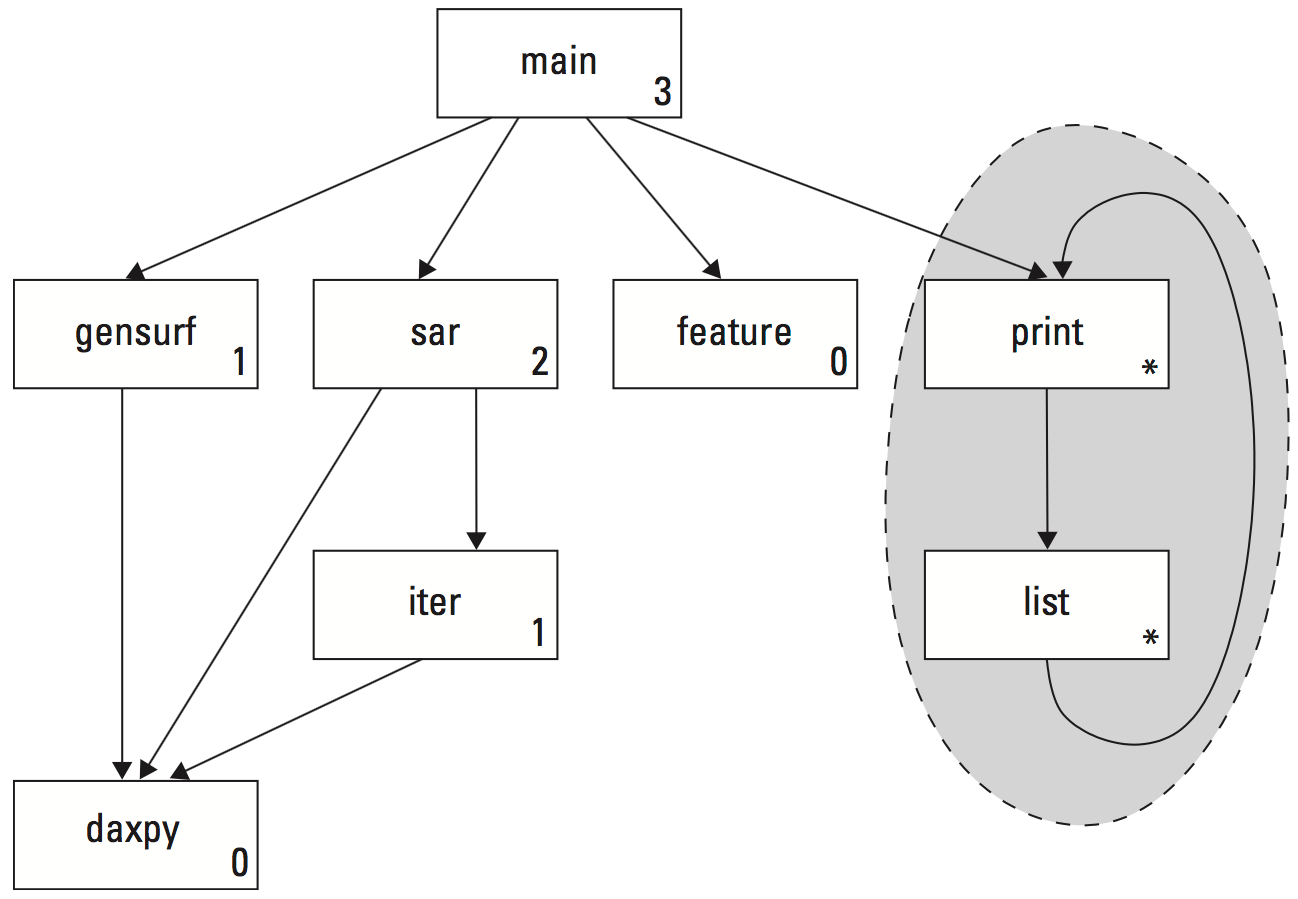
\includegraphics[width=0.8\textwidth]{img/f4-4.png}
	\caption{}
	\label{fig:f4-4}
\end{figure}

O exemplo da Figura \ref{fig:f4-4} mostra que as funções \texttt{print} e \texttt{list} formam um componente fortemente conectado e são marcados com um *. Em seguida, os vértices restantes de $ G $ são assinalados por uma regra ordinal,

$$
\text{ord}(u) = 
\left\{\begin{matrix}
0 & \text{se nó} u \text{é uma folha} \\ 
\underset{(u,v) \in E(G)}{\max} \{ \text{ord}(v) \} + 1 & \text{caso contrário}
\end{matrix}\right.
$$



\subsubsection{Modelo \textit{Multithread}}

Além do modelo coprocessado, tem-se o modelo \textit{multithreads} que emerge como uma importante técnica de programação utilizada até em computadores com multiprocessadores. Neste modelo, o paralelismo natural do \textit{hardware} é conhecido e o designer reconhece que o processador e os componentes executam continuamente. A coordenação desses componentes é manuseada por comunicações primitivas que tem sido desenvolvidas por processo concorrentes como semáforos, mensagens e outros. Cada \textit{hardware} é considerado um componente que executa como uma \textit{thread} paralela e o sistema de semáforos é utilizado para deixar o sistema consistente e assim, ao invés de bloqueado, o \textit{hardware} conceitualmente fica em bloqueio esperado pelo semáforo ou por uma mensagem.



\subsubsection{Modelo de Rede em Chip}

Este modelo investiga o estado distribuído completamente e depende da troca de mensagem para explicitar o estado. A coordenação é implícita com a transferência de estado. Como é assumido que o design referencial de \textit{software} foi construído com comandos de troca de mensagem explícita, não se considera em um manual de sistemas embarcados. Entretanto, tem-se visto que técnicas de alta-performance continuam filtrando-se para o nível de sistemas embutidos.



\subsection{Transferência de Estado}

Manter estado consistente sobre dispositivos FPGA e processadores é um desafio. Isso pois, cada FPGA tem sua própria hierarquia de memória independente, estados são amplamente distribuídos no design, e há ampla variedade de interconexões entre FPGA e processadores significando menos estados para serem transferidos e grande variedade de mecanismos disponíveis. Para entender melhor deve-se definir dois conceitos sendo eles estado afetado e preso ajudando a decidir quais partes do estado da aplicação necessitam de ser explicitamente comunicados entre processador e recurso.



\subsubsection{Estado Afetado}

Na computação alguns estados são independentes pela construção e não precisam de ser transferidos. Retirando tais estados, restam somente os estados afetados no qual são os dados da aplicação que, durante a transferência de controle, podem ser modificados ou litros por um recurso ou processador, necessitando de ser consistente.



Estados afetados podem existir em grande escala principalmente quando arranjos, estruturas de dados complexas ou ponteiro estão envolvida e podem ser acessados de várias formas possíveis e geralmente não é possível saber se dois ponteiros estão apontando para um mesmo endereço.



\subsubsection{Estado Preso}

Quando parte da hierarquia de memória é compartilhada, nem todo o dado tem que ser explicitamente transferido. Computadores modernos são construídos com quantidade significativa de memória pode ser utilizada como parte de estado sem a atualização da memória primária. Compiladores naturalmente utilizam toda a vantagem de registradores para armazenar estados, implementações em \textit{hardware} incorporam dados ao longo do projeto e seus registradores e \textit{flip-flops} possuem valores intermediários entre ciclos de \textit{clock} dentro do projeto. O estado de uma aplicação é armazenado em várias partes do sistema. Para um recurso implementar parte de uma aplicação, precisa-se integrar com parte do estado. Esse pode ser considerado mais facilitado pelo fato de que o estado está localizado em um espaço comum mas se um estado está localizado num registrador ou em uma cache de um processador, ele não pode ser acessado pelo sistema externo e, neste caso, o estado encontra-se preso e deve ser explicitamente transmitido pela interface.



\subsubsection{Problema de Transferência de Estado}

Estados afetados que são presos necessitam de ser explicitamente comunicados e é feito por um processo chamado \textit{marshaling}, realizando o processo de \textit{marshaling} grupos de elementos de um estado afetado de uma aplicação em registros lógicos que são explicitamente transferidos. Tendo a premissa que o processador tem o controle inicial, tem-se quatro tipos de registros que podem ser utilizados. Os dois primeiros são utilizados para iniciar e outro para finalizar a transferência de um conjunto de elementos para o recurso sendo eles \textit{Type-I} e \textit{Type-F}. Os outros dois tipos de \textit{marshal} são utilizados repetidamente e são utilizados quando o recurso é invocado, \textit{Type-CI}, e quando é completado \textit{Type-CO}. Um exemplo da diferença entre \textit{Type-F} é quando se tem um \textit{core} que acumula um valor em uma variável global. O registro \textit{Type-F} seria utilizado para ler o valor da variável após sua última invocação \textit{Type-CO}.



Um processo de tradução pode ser incorporado com o \textit{marshaling}, sendo o exemplo o processo de conversão de ponto flutuante para fixo. O grupo de elementos é lógico pelo fato do \textit{assembly} não significar estritamente que os elementos são copiados para uma memória de locação contínua. 



A forma mais simples de transferir estados são copiando os registros, parar o processador enquanto o recuso processa. Este é chamado de empurrar (\textit{push}) os dados no qual transmite o dado antes da transferência do controle. Caso registro já existe e é conhecido, é feito a transferência de controle e o recurso realiza o puxar (\textit{pulls}) dos dados. Situações onde o estado afetado é maior que o dado a ser utilizado, utiliza-se de interfaces.



Em geral, a escolha da transferência por instância ou por continuação é determinada por uma meta do recurso. Instâncias são utilizadas quando deseja-se reduzir a latência de tarefas e transferir pequenos registros. Continuações são para aumentar a vazão de dados e a redução de latência não é possível ou não suficiente boa. Esta geralmente envolve a configuração de transferências DMA e a incorporação de \textit{buffers} FIFO no qual pode aumentar a área e em algumas situações a latência.



As melhores implementações em \textit{hardware} utilizam formatos diferentes de estruturas de dados. Traduções são item integral para dados \textit{marshal}.



Esclarecido os conceitos fundamentais, será descrito a abordagem formal para o problema de particionamento.



\section{Questões Práticas}

\subsection{Questões de \textit{Profiling}}

Uma suposição não adequada com a formulação analítica é que ela usa informação de \textit{profile} para aproximar o tempo de fração que uma aplicação gasta em uma sub-rotina ou bloco básico, mas no entanto, várias situações podem gerar resultados enganosos.



\subsubsection{Execução Dependente de Dados}

Quanto um simples conjunto de dados não representa o tempo gasto de cada sub-rotina quando este é alterado a sub-rotina não terá mudanças substanciais com a mudança do dado de entrada. A detecção da situação onde um único conjunto de dados não é representativo torna a situação difícil e requer que o designer do sistema compreenda a operação fundamental da aplicação como é o caso da análise de complexidade das rotinas. É possível analisar esses casos com alguns métodos sendo a análise manual dos algoritmos e suas operações básicas, a coleta de informações \textit{profiling} baseado em diferentes conjuntos de dados ou mesmo a tentativa de separar a aplicação talvez ao longo dos limites do módulo e fazer o \textit{profile} de cada módulo independente.



\subsubsection{Comportamento Correlacionado}

Outra questão surge em aplicações que explicita o uso de eventos cronometrados. Muitos \textit{profile} assumem que a aplicação fará um progresso estável em direção à solução mas algumas aplicações incorporam o tempo. Sistemas de \textit{profiles} usam um temporizador de intervalo para amostrar o contador de programas dependendo da aplicação para não serem correlacionados estatisticamente com o temporizador. No entanto, se a aplicação possui operações executando em tempos regulares, periódicos, então os resultados do \textit{profiling} podem ser considerado enganosos. Por exemplo, se uma aplicação é executada a cada 10ms e a amostragem é feita a cada 10ms, então o \textit{profiler} não fornecerá dados concretos referentes ao sistema.



\subsubsection{Comportamento Faseado}

Sobre a totalidade de sua execução, o controle se move entre \textit{clusters} de operações relacionadas, isso é, a execução de uma aplicação exibida localmente. Como um exemplo, consideremos uma aplicação que possui três rotinas. Assumindo que cada possui $ 33\% $ de tempo de execução, e que cada tem a possibilidade de ter um \textit{speed up} de 50\% e postas de forma ordenada da primeira à última. Se existe espaço somente para uma rotina em recursos de FPGA, então o \textit{speed up} máximo será de 12\%. Mas se o comportamento faseado é suportado pelo design de sistema, então há mais opções. Um é olhar procurar itens em comum sobre os três \textit{cores} e uma segunda é um \textit{hardware} multiplexado por tempo. Não há abordagens automáticas para esse.



\subsubsection{Efeitos de I/O}

\textit{Profiles} não contam tempo de I/O tais como acesso ao espaço de usuário e dispositivos realizando algum procedimento de busca ou ação.



\subsubsection{Números de Chamada}

\textit{Profiles} entretanto continuará a calcular quando sub-rotinas são invocadas. É importante ter noção o quanto uma sub-rotina é invocada.



\subsection{Estrutura de Dados}

Design de referência de \textit{software} naturalmente reflete um viés em relação às implementações em \textit{software}. Isso é compreensível, já que a programação é ensinada no contexto de modelo de computação sequencial ordinário. Com esses modelos, a diferença entre 

\begin{verbatim}
while( i!=NULL ) {
  proc(i) ;
  i = i->next ;
} 
\end{verbatim}
e 
\begin{verbatim}
while( i<n ) {
 proc(x[i]) ;
 i=i+1;
}
\end{verbatim}

é insignificante já que ambos tomam $ \mathcal{O}(n) $ passos, mas em nível de \textit{hardware} o último pode ser mais desejável sendo no mínimo, uma ampla janela de pré-busca é possível. Se pudermos determinar que, em várias iterações do ciclo, cada \texttt{proc(x[i])} é independente, então pode-se melhorar o design por meio de \textit{pipeline} ou paralelismo regular.

O design de referência de \textit{software} serve como extremamente bem como uma especificação, mas se executar um \textit{profile} do design de referência, não será capturado os benefícios da implementação pois esses benefícios provêm de alterações algorítmicas e são improváveis de serem reveladas por técnicas automáticas. Consequentemente, cai sobre o designer de sistema compreender ambos o algoritmo de \textit{software} implementado no design referencial e como pode ser re-implementado em \textit{hardware}.

Há vários formas comuns de estruturas de \textit{software} que pode ser rearranjadas para produzir melhor design de \textit{hardware}. Estruturas de dados que utilizam ponteiro como listas encadeadas, árvores, etc. podem ser representadas por uma estrutura ``\textit{flat}'' como vetores e arranjos produzindo acesso regular em memória que podem ser pré-buscadas subsequentemente ou utilizadas em \textit{pipeline}. Outra forma de ganho de performance é no tamanho de bit. Programadores de \textit{software} geralmente assumem um valor fixo, mesmo que utilizem somente poucos bits de informação. Enquanto \textit{software} tem caminho de dados fixos e relativamente baixa largura de banda entre componentes, \textit{hardware} se destaca no gerenciamento de largura de bits arbitrárias sendo possível alavancar grande largura de banda fornecida pela interconexão programável do FPGA.



\subsection{Manipulando Tamanho de Recurso}

A mudança mais simples envolver quebrar uma sub-rotina em sub-rotinas menores fazendo com que o recurso em \textit{hardware} fique menor e mais fácil de ser implementado.



Há três momentos que agregar sub-rotinas são necessárias. Se duas sub-rotinas tomam 25\% cada uma do tempo da aplicação, então elas são candidatos fortes para a implementação em \textit{hardware}. No entanto, se for implementado individualmente, cada uma invoca o custo da sua interfaceação. Se há três sub-rotinas relacionadas (uma invocando a próxima), então a combinação delas pode reduzir o custo de invocações. Entretanto, o custo da interface não é sempre insignificante e vale a pena o esforço do usuário para investigar a situação.



Qualquer outra mudança é substancial. Frequentemente, implementação em \textit{hardware} tem performance significativa por ter formato de dados de dados específicos da aplicação. Para que o \textit{software} seja mais eficiente nos formato de dados não padronizados, programadores irão investir em estruturas de dados que não são bem mapeadas para o \textit{hardware}. Assim, vale a pena olhar para o propósito e considerar a substituição de estruturas de dados para melhor explorar o \textit{hardware}.

